\documentclass{article}
\usepackage{graphicx}
\usepackage[margin=1.5cm]{geometry}
\usepackage{amsmath}

\begin{document}
\twocolumn

\title{Tuesday Warm Up, Unit 0: Foundations and Fundamentals}
\author{Prof. Jordan C. Hanson}
\maketitle

\section{Memory Bank}

\begin{itemize}
\item $\sqrt{-1} = j$ ... The fundamental imaginary unit.
\item $z = x + jy$ ... A complex number.
\item $\Re \lbrace z \rbrace = x$, $\Im \lbrace z \rbrace = y$ ... Real and imaginary parts.
\item $z^{*} = x - j y$ ... The complex conjugate of $z$.
\item $|z| = \sqrt{z z^{*}} = \sqrt{x^2 + y^2}$ ... The magnitude of $z$.
\item $\tan\phi = y/x$ ... The phase angle of $z$.
\item $|z| = r$, so $x = r\cos\phi$, and $y = r\sin\phi$.
\item \textbf{Complex response $R(f)$ of a high-pass filter with resistance $r$ and capacitance $C$:} \\ $R(f) = j\omega\tau/(1+j\omega \tau)$, where $\omega = 2\pi f$, and $\tau = rC$.
\end{itemize}

\section{Application of Complex Numbers: AC Circuit Filters}

\begin{enumerate}
\item The response of a simple high-pass RC filter is
\begin{equation}
R(f) = j\omega\tau/(1+j\omega \tau) \label{eq:1}
\end{equation}
(See memory bank).  (a) Find the magnitude\footnote{Hint: multiply the top and bottom by the complex conjugate of the denominator.} of Eq. \ref{eq:1}.  (b) Find the phase angle of Eq. \ref{eq:1}. (c) Graph the magnitude and phase angle versus frequency, by hand.  (d) Suppose a signal has a an amplitude of $A$ at a frequency $f$: $A(f)$.  The filtered amplitude is $R(f) A(f)$.  If $A=1$ at $f = 0.5$ kHz, $R = 1$ k$\Omega$, and $C = 1$ $\mu$F, what is the filtered amplitude $A(f) R(f)$?\footnote{This filtered amplitude is a result of the \textit{convolution theorem}, which we will encounter in a later chapter.} \\ \vspace{4cm}
\end{enumerate}

\section{Statistics, Probability, Noise, and ADC/DAC}

\begin{enumerate}
\item Consider the sampled, digitized signal in Fig. \ref{fig:1}, with quantization error shown in Fig. \ref{fig:2}.  Note that when the signal is \textit{digitized}, the error in voltage is equally likely to fall anywhere between two digital voltage levels: $[-1/2,1/2]$ LSB (least significant bit).  The error distribution is shown by the PDF on the right side of Fig. \ref{fig:2}.  (a) If the signal ranges between 0 and 3.3 Volts, and there are 10 bits available for digitization ($2^10 = 1024$ voltage levels), what is the voltage per level? (b) The voltage per level is called the LSB, or \textit{least significant bit.} What is the LSB in millivolts? (c) What is the average quantization error in LSB?  (d) What is the standard deviation of the quantization error in LSB?
\end{enumerate}

\begin{figure}
\centering
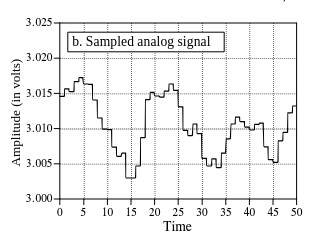
\includegraphics[width=0.24\textwidth]{quant_1.png}
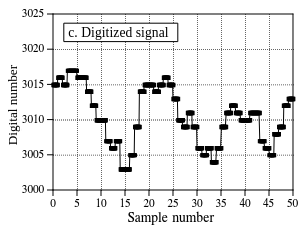
\includegraphics[width=0.24\textwidth]{quant_2.png}
\caption{\label{fig:1} (Top) A sampled, analog signal. (Bottom) The data from (top), but digitized.}
\end{figure}
\begin{figure}
\centering
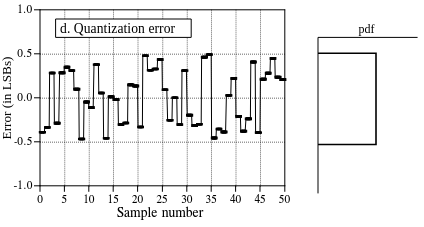
\includegraphics[width=0.35\textwidth]{quant_3.png}
\caption{\label{fig:2} The quantization error for the signal in Fig. \ref{fig:1}.}
\end{figure}

\end{document}
